%!TeX encoding = UTF-8 Unicode
\documentclass{article}
\usepackage[pdftex]{graphicx} %for embedding images
\usepackage{url} %for proper url entries
\usepackage[bookmarks, colorlinks=false, pdfborder={0 0 0}, pdftitle={Laboratory ML Project 02}, pdfauthor={Nhut-Nam Le}, pdfsubject={Introduction to Machine Learning}, pdfkeywords={report, exercises}]{hyperref} %for creating links in the pdf version and other additional pdf attributes, no effect on the printed document
%\usepackage[final]{pdfpages} %for embedding another pdf, remove if not required
\usepackage[utf8]{inputenc}
\usepackage[english, vietnamese]{babel}
\usepackage{float}
\usepackage{fancyhdr}
\usepackage{pythonhighlight}
\usepackage[left=3cm, right=3cm, top=2cm, bottom=2cm]{geometry}
\usepackage{parskip}
\usepackage{tikz}
\usepackage{hyperref}
\usepackage[]{algorithm2e}
\usepackage[noend]{algpseudocode}
\usepackage{amsmath}
\usepackage{amsfonts}

\usepackage{listings}
\usepackage{color}

\definecolor{dkgreen}{rgb}{0,0.6,0}
\definecolor{gray}{rgb}{0.5,0.5,0.5}
\definecolor{mauve}{rgb}{0.58,0,0.82}

\newcommand\T{\rule{0pt}{2.6ex}}       % Top strut
\newcommand\B{\rule[-1.2ex]{0pt}{0pt}} % Bottom strut


\lstset{frame=tb,
	language=Java,
	aboveskip=3mm,
	belowskip=3mm,
	showstringspaces=false,
	columns=flexible,
	basicstyle={\small\ttfamily},
	numbers=none,
	numberstyle=\tiny\color{gray},
	keywordstyle=\color{blue},
	commentstyle=\color{dkgreen},
	stringstyle=\color{mauve},
	breaklines=true,
	breakatwhitespace=true,
	tabsize=3
}

\setlength{\parindent}{15pt}
\setlength{\headheight}{15.2pt}
\pagestyle{fancy}
\lhead[<even output>]{NHẬP MÔN HỌC MÁY}
\rhead[<even output>]{BÁO CÁO ĐỒ ÁN THỰC HÀNH 02}
\title{research-outline}
\author{Nhut-Nam Le}
\date{2021}
\begin{document}
	\begin{titlepage}
		\begin{center}
			% Top of the page
			\large{\textbf{ĐẠI HỌC KHOA HỌC TỰ NHIÊN, ĐHQG-HCM\\KHOA CÔNG NGHỆ THÔNG TIN\\BỘ MÔN KHOA HỌC MÁY TÍNH}}\\
			
\includegraphics[width=0.75\textwidth]{images/khtn.png}\\
			% Title
			\large \textbf{NHẬP MÔN HỌC MÁY}\\[0.1in]
			\huge \textbf{BÁO CÁO ĐỒ ÁN THỰC HÀNH}\\[0.1in]
			\huge \textbf{CLASSIFICATION - PHÂN LỚP}\\[0.1in]
			\vfill
			\normalsize
			% Submitted by
			\normalsize
			% Lecturers
			\textbf{Giảng viên lý thuyết}\\
			{\textbf{TS.} Bùi Tiến Lên}\\[0.1in]
			% Teacher Assistant
			\textbf{Giảng viên hướng dẫn}\\
			\vspace{0.1in}
			{Dương Nguyễn Thái Bảo, Nguyễn Ngọc Đức, Nguyễn Tiến Huy, Lê Thanh Phong}\\[0.1in]
			\textbf{Sinh viên thực hiện} \\
			\vspace{0.1in}
			% Submitted by
			{Vương Gia Bảo, Ngô Xuân Kiên, Lê Nhựt Nam, Nguyễn Viết Dũng}\\[0.1in]
			% Date time when written report
			\vfill
			Tháng 5 năm 2021
		\end{center}
	\end{titlepage}
	\newpage
	% End Title4
	
	\pagenumbering{roman} %numbering before main content starts
	\cleardoublepage
	%\pagebreak
	\phantomsection
	\addcontentsline{toc}{section}{Lời cảm ơn}
	\section*{Lời cảm ơn}
	\vspace{1.0in}
	\begingroup
	\setlength{\parindent}{0pt}
	\qquad Trong quá trình thực hiện đồ án này, chúng em đã nhận được rất nhiều sự giúp đỡ cũng như hỗ trợ từ các thầy cô Trường Đại học Khoa học Tự nhiên, ĐHQG-HCM và các bạn bè trong lớp Nhập môn Học Máy. Chúng em xin bày tỏ lòng cảm ơn chân thành đến mọi người vì đã giúp đỡ hướng dẫn, chỉ bảo rất tận tình.
	
	\qquad Đặc biệt, chúng em xin bày tỏ lòng biết ơn sâu sắc đến các thầy cô khoa Công nghệ Thông tin, cụ thể hơn là thầy Bùi Tiến Lên và các thầy hướng dẫn đã giảng dạy rất nhiệt, cung cấp nhiều slides, tài nguyên học tập cần thiết, tạo điều kiện tốt nhất để chúng em có thể hoàn thành được đồ án này.
	
	\qquad Trong quá trình, viết báo cáo này, chúng em không thể tránh khỏi nhiều thiếu sót, hy vọng mong nhận được góp ý từ thầy để chúng em tiếp tục hoàn thiện hơn đối với đồ án này, cũng như rút kinh nghiệm cho những đồ án, những báo cáo kế tiếp.
	
	\vspace{1.0in}
	\textbf{Đại học Khoa học Tự nhiên, ĐHQG-HCM.}\\
	Vương Gia Bảo, Ngô Xuân Kiên, Lê Nhựt Nam, Nguyễn Viết Dũng\\
	Tháng 4 năm 2021\\
	\endgroup
	
	\newpage
	\tableofcontents
	\newpage
	\pagenumbering{arabic} %reset numbering to normal for the main content
	\setcounter{secnumdepth}{0}
	
	\section{Thông tin nhóm}
	\begin{table}[H]
		\centering
		\begin{tabular}{ | p{1cm} |  p{3cm} | p{5cm} | p{5cm}  |}\hline
			STT	& MSSV & Họ tên đầy đủ & Email liên lạc \\\hline
			1 & 18120009 & Vương Gia Bảo & 18120009@student.hcmus.edu.vn  \\ \hline
			2 & 18120045 & Ngô Xuân Kiên & 18120045@student.hcmus.edu.vn \\ \hline
			3 & 18120061 & Lê Nhựt Nam & 18120061@student.hcmus.edu.vn  \\ \hline
			4 & 18120167 & Nguyễn Viết Dũng &  18120167@student.hcmus.edu.vn \\ \hline
		\end{tabular}
	\end{table}
	\section{Phân công công việc}
	\begin{table}[H]
		\begin{tabular}{ | l | l | l | p{5.5cm} | p{3cm} |}
			\hline
			STT & MSSV & Họ tên & Nội dung công việc & Mức độ hoàn thành  \\ \hline
			1 & 18120009 & Vương Gia Bảo & Thu thập dữ liệu, đọc hiểu source, báo cáo Introduction Paper &  100\%\T\B\\ \hline
			2 & 18120045 & Ngô Xuân Kiên & Thu thập dữ liệu, đọc hiểu source, báo cáo Related Work Paper & 100\%\T\B \\ \hline
			3 & 18120061 & Lê Nhựt Nam & Thu thập dữ liệu, đọc hiểu source, báo cáo, SincNet Architecture, Slides thuyết trình, Midterm Report & 100\%\T\B \\ \hline
			4 & 18120167 & Nguyễn Viết Dũng &  Thu thập dữ liệu, đọc hiểu source, báo cáo experimental setup Paper & 100\%\T\B \\ \hline
		\end{tabular}
	\end{table}
	\section{Tiêu chí đánh giá đồ án}
	\subsection{Bảng tiêu chí cho đồ án}
	\begin{table}[H]
		\begin{tabular}{ | p{5cm} | p{6.25cm} | p{3cm} |}\hline
			Tên tiêu chí đồ án & Nội dung tiêu chí & Mức độ hoàn thiện  \T\B\\\hline
			Nhận diện bài toán & Sinh viên cần tìm hiểu bài toán và dữ liệu được giao
			nhằm xác định nội dung và ý nghĩa bài toán thực tế cần giải quyết. Thông
			qua đó, sinh viên có khả năng ánh xạ vấn đề thực tế sang bài toán lập trình & 100\%  \T\B\\\hline
			Giải quyết vấn đề & Sinh viên được yêu cầu đưa ra các giải pháp và hướng
			tiếp cận nhằm giải quyết được yêu cầu bài toán thực tế & 100\%  \T\B\\\hline
			Xử lý và phân tích dữ liệu & Sinh viên có khả năng xử lý các công cụ phân
			tích dữ liệu tự động nhằm tìm ra các thông tin hữu ích, các đặc trưng tiềm ẩn
			ảnh hưởng để mục tiêu bài toán &100\%  \T\B\\\hline
			Thiết kế và cài đặt các thuật toán máy học & Sinh viên được yêu cầu có
			khả năng đề xuất, triển khai và giải thích các thuật toán máy học nhằm giải
			quyết bài toán được giao & 100\%  \T\B\\\hline
		\end{tabular}
	\end{table}
	\subsection{Bảng yêu cầu cho đồ án}
	\begin{table}[H]
		\begin{tabular}{ | p{5cm} | p{6.5cm} | p{3cm} |}\hline	
			Tên yêu cầu & Nội dung yêu cầu & Mức độ hoàn thiện  \T\B\\\hline
			Phân tích dữ liệu & Phân tích kỹ bài toán và tập dữ liệu hình ảnh được cung cấp. Chọn lựa và
			trình bày kiểu mạng nơron để giải quyết bài toán. & 100\%  \T\B\\\hline
			Cài đặt thuật toán & Cài đặt mạng Nơron. & 100\%  \T\B\\\hline
			Trình bày kết quả và nhận xét & Báo cáo kết quả đạt đưoc sau quá trình phân tích và cài đặt. & 100\%  \T\B\\\hline
		\end{tabular}
	\end{table}	
	\section{Nội dung báo cáo}
	\section{1. Tổng quan về bài toán}
	\qquad Trong nộng nghiệp, năng suất của cây trồng phụ thuộc rất nhiều vào thời
	tiết, chế độ chăm sóc, sâu bệnh,... để tăng năng suất người trồng cần có những
	biện pháp hạn chế những tác động của các yếu tố trên.
	
	Tuy nhiên, bản thân cây trồng cũng có những loại bệnh nhất định và thường
	biểu hiện ra bên ngoài trên thân, lá... những biểu hiện đó bất thường trên cây
	trồng thường liện quan tới một loại bệnh nào đó.
	
	Nhằm giúp người trồng xác định được loại bệnh đang có trên cây trồng,
	sinh viên được cung cấp tập dữ liệu hình ảnh về các loại bệnh trên cây và tập dữ
	liệu đã được xác định được loại bệnh (train.csv và test.csv) bao gồm 4 loại:
	\begin{itemize}
		\item Healthy
		\item Combinations
		\item Rust
		\item Scab
	\end{itemize}
	Dữ liệu có 3 tập tin
	\begin{itemize}
		\item train.csv
		\begin{itemize}
			\item image\_id: the foreign key
			\item combinations: one of the target labels
			\item healthy: one of the target labels
			\item rust: one of the target labels
			\item scab: one of the target labels
		\end{itemize}
		\item test.csv
		\begin{itemize}
			\item image\_id: the foreign key
		\end{itemize}
		\item sample\_submission.csv
		\begin{itemize}
			\item image\_id: the foreign key
			\item combinations: one of the target labels
			\item healthy: one of the target labels
			\item rust: one of the target labels
			\item scab: one of the target labels
		\end{itemize}
	\end{itemize}
	Thư mục images chứa tất cả ảnh huấn luyện (train images) và ảnh kiểm tra (test images), với định dạng là .jpg
	\section{2. Công cụ và môi trường thực thi}
	\qquad Với yêu cầu thực hiện của đồ án, để thuận tiện cho làm việc, trao đổi, nhóm chọn môi trường Google Colab hỗ trợ để chạy Jupyter Notebook, mặc khác là để đảm bảo rằng đầy đủ các thư viện cần thiết cho đồ án.
	
	Đối với tác vụ tính toán số học, xử lý bảng dữ liệu, nhóm chọn hai thư viện mạnh mẽ, Numpy và Pandas hỗ trợ trong việc đọc các đường dẫn, tính toán kernel, ...
	
	Đối với tác vụ khai thông tin, phân tích dữ liệu bằng các công cụ trực quan hóa dữ liệu, nhóm sử dụng thư viện Matplotlib, Seaborn và Plotly trong việc vẽ các biểu đồ (chart), sơ đồ (diagram), histogram,...
	
	Đối với tác vụ đọc, ghi, xử lý dữ liệu hình ảnh, nhóm chọn thư viện Python-OpenCV, scikit-image để triển khai các phép biến đổi tăng cường hình ảnh như phát hiện biên cạnh bằng giải thuật Canny (The Canny Edge Detector), Đóng bouding boxes, Lật ảnh (Flipping image), Làm trơn hình ảnh (Bluring), Phép tính chập với kernel tùy chọn (Convolutional), ...
	
	Đối với tác vụ cài đặt Neural Networks, nhóm chọn thư viện Pytorch sử dụng GPU Google Colab trong việc cài đặt mô hình mạng, huấn luyện mô hình
	
	Đối với tác vụ đánh giá mô hình, nhóm sử dụng Sklearn hỗ trợ sử dụng một số độ đo trong việc đánh giá mô hình.
	
	\section{3. Khám phá cấu trúc dữ liệu}
	\begin{figure}[H]
		\centering
		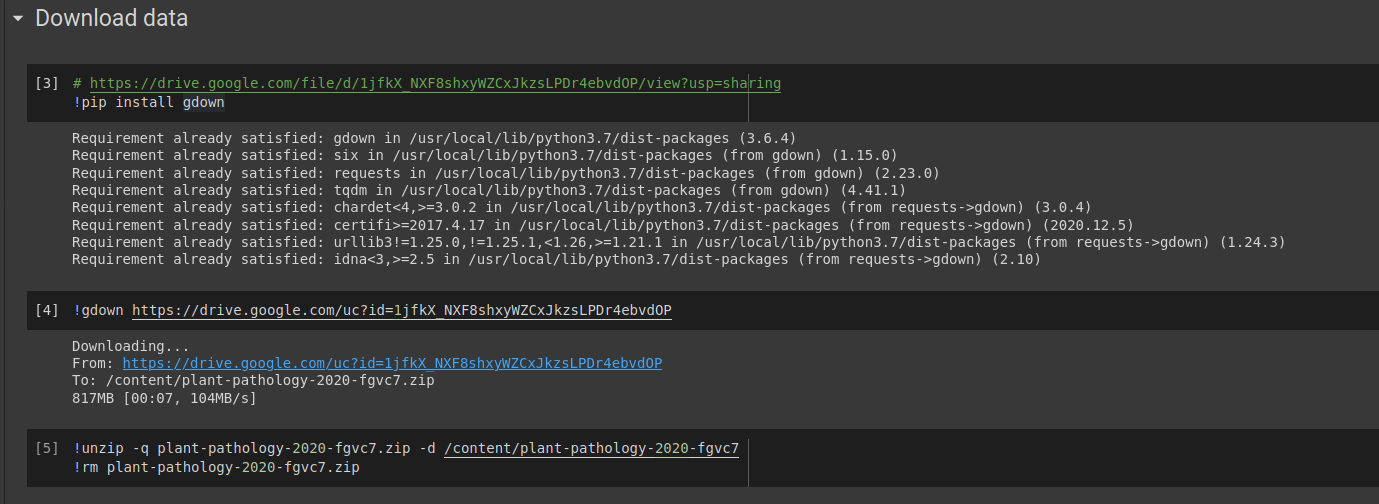
\includegraphics[width=0.75\linewidth]{images/download_plant_pathology_dataset.png}
		\label{fig:writing-thesis}
	\end{figure}
	\begin{figure}[H]
		\centering
		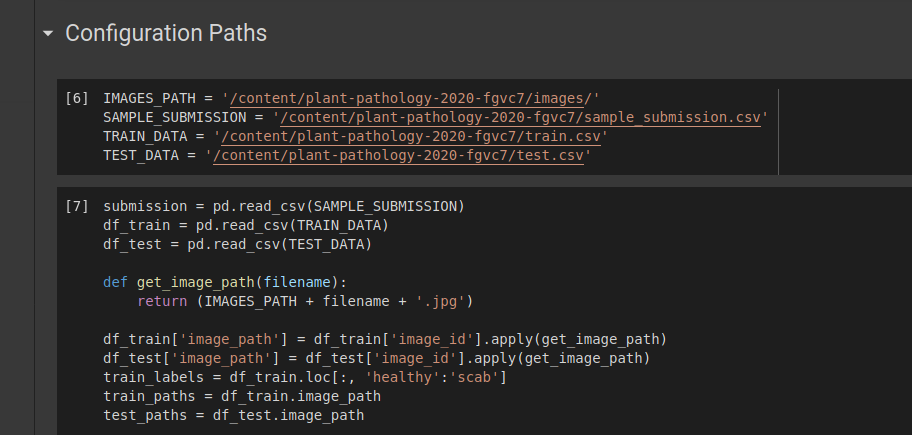
\includegraphics[width=0.75\linewidth]{images/configuration_paths.png}
		\label{fig:writing-thesis}
	\end{figure}
	\begin{figure}[H]
		\centering
		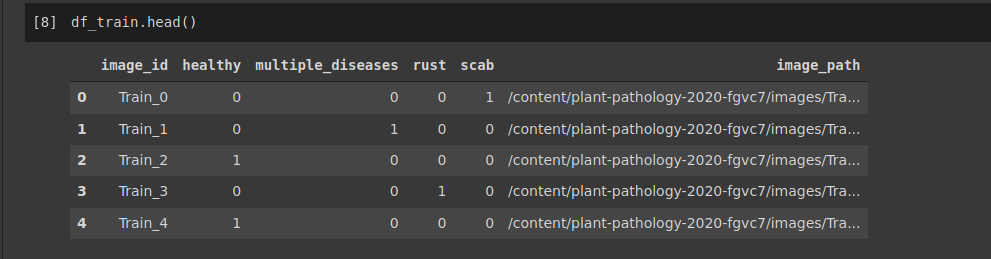
\includegraphics[width=0.75\linewidth]{images/head_df_train.png}
		\label{fig:writing-thesis}
	\end{figure}
	\begin{figure}[H]
		\centering
		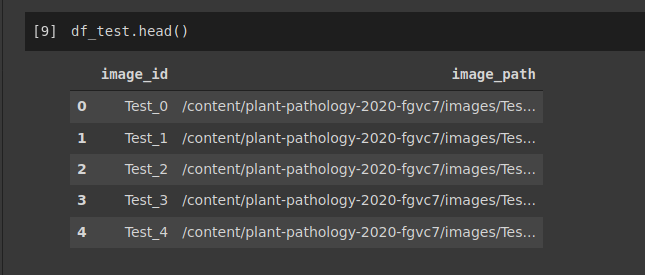
\includegraphics[width=0.75\linewidth]{images/head_df_test.png}
		\label{fig:writing-thesis}
	\end{figure}
	
	\section{4. Trực quan và phân tích dữ liệu}
	\subsection{4.1 Tổng quan về hình ảnh các loại bệnh}
	\textbf{Chọn ngẫu nhiên những chiếc lá không bị bệnh - Healthy Leaf}
	\begin{figure}[H]
		\centering
		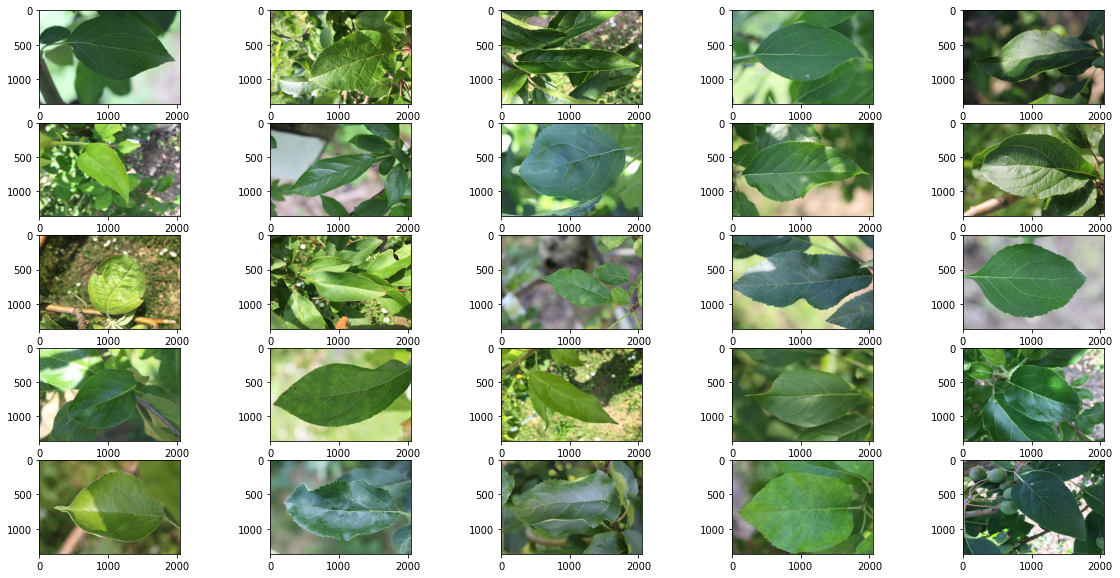
\includegraphics[width=1\linewidth]{images/sample_healthy_leaf.png}
		\caption{Một số mẫu hình ảnh về Healthy Leaf}
		\label{fig:writing-thesis}
	\end{figure}
	\begin{python}
		def plot_patches(data, size_selection, width_size, height_size, figure_size, type_patches=0, is_positive=True):
		fig, ax = plt.subplots(height_size, width_size, figsize=figure_size)
			if type_patches == 0:
				if is_positive:
					healthy_selection = np.random.choice(
					data[data.healthy == 1].index.values, size=size_selection, replace=False)
					for i in range(height_size):
						for j in range(width_size):
						idx = healthy_selection[j + width_size*i]
						image = io.imread(data.loc[idx, 'image_path'])
						ax[i, j].imshow(image)
					ax[i, j].grid(False)
				else:
					non_healthy_selection = np.random.choice(
					data[data.healthy == 0].index.values, size=size_selection, replace=False)
					for i in range(height_size):
						for j in range(width_size):
							idx = non_healthy_selection[j + width_size*i]
							image = io.imread(data.loc[idx, 'image_path'])
							ax[i, j].imshow(image)
							ax[i, j].grid(False)
	\end{python}
	\textbf{Chọn ngẫu nhiên những chiếc lá bị bệnh tổ hợp - Multiple Diseases Leaf}
	\begin{figure}[H]
		\centering
		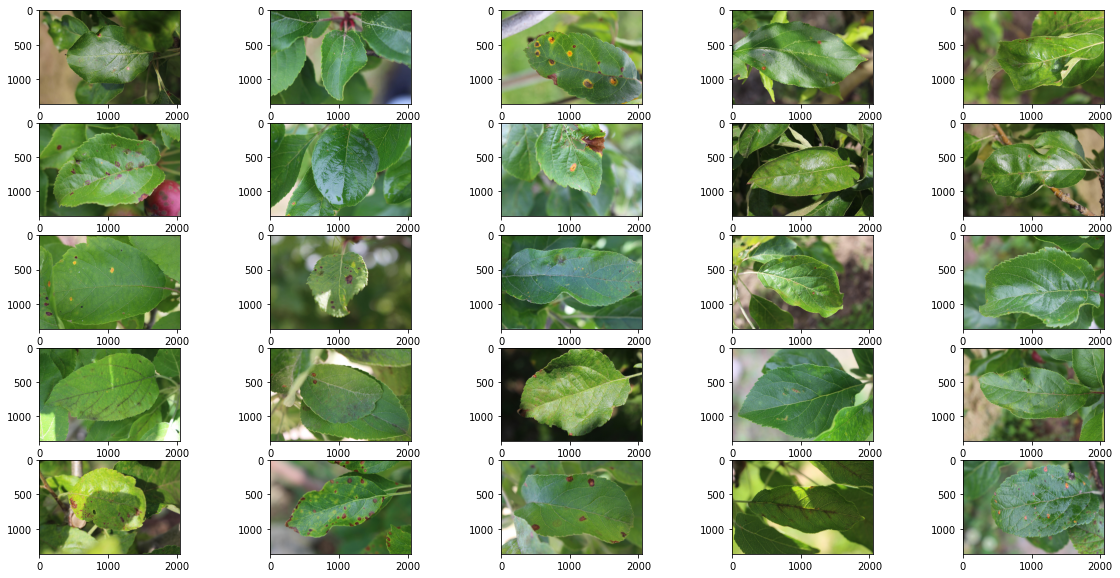
\includegraphics[width=1\linewidth]{images/sample_multiple_diseases_leaf.png}
		\caption{Một số mẫu hình ảnh về Multiple Diseases Leaf}
		\label{fig:writing-thesis}
	\end{figure}
	\begin{python}
		def plot_patches(data, size_selection, width_size, height_size, figure_size, type_patches=0, is_positive=True):
			if type_patches == 1:
				if is_positive:
				multiple_diseases_selection = np.random.choice(
				data[data.multiple_diseases == 1].index.values, size=size_selection, replace=False)
				for i in range(height_size):
					for j in range(width_size):
						idx = multiple_diseases_selection[j + width_size*i]
						image = io.imread(data.loc[idx, 'image_path'])
						ax[i, j].imshow(image)
						ax[i, j].grid(False)
				else:
					non_multiple_diseases_selection = np.random.choice(
					data[data.multiple_diseases == 0].index.values, size=size_selection, replace=False)
					for i in range(height_size):
						for j in range(width_size):
							idx = non_multiple_diseases_selection[j + width_size*i]
							image = io.imread(data.loc[idx, 'image_path'])
							ax[i, j].imshow(image)
							ax[i, j].grid(False)
	\end{python}
	\textbf{Chọn ngẫu nhiên những chiếc lá bị bệnh Rust - Rust Diseases Leaf}
	\begin{figure}[H]
		\centering
		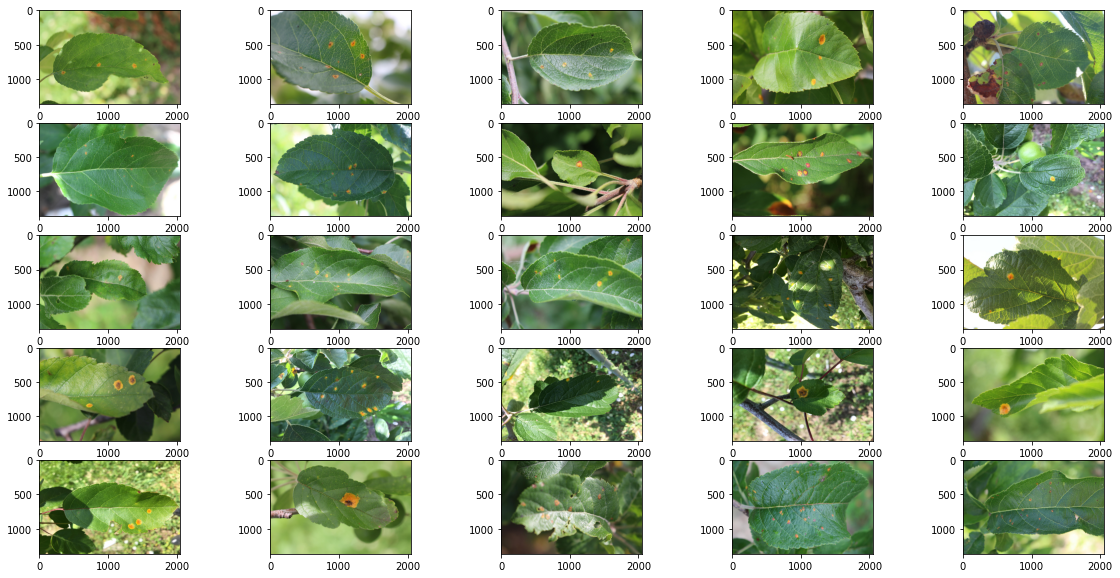
\includegraphics[width=1\linewidth]{images/sample_rust_leaf.png}
		\caption{Một số mẫu hình ảnh về Rust Diseases Leaf}
		\label{fig:writing-thesis}
	\end{figure}
	\begin{python}
		def plot_patches(data, size_selection, width_size, height_size, figure_size, type_patches=0, is_positive=True):
			if type_patches == 2:
				if is_positive:
					rust_selection = np.random.choice(
					data[data.rust == 1].index.values, size=size_selection, replace=False)
					for i in range(height_size):
						for j in range(width_size):
							idx = rust_selection[j + width_size*i]
							image = io.imread(data.loc[idx, 'image_path'])
							ax[i, j].imshow(image)
							ax[i, j].grid(False)
				else:
					non_rust_selection = np.random.choice(
					data[data.rust == 0].index.values, size=size_selection, replace=False)
					for i in range(height_size):
						for j in range(width_size):
							idx = non_rust_selection[j + width_size*i]
							image = io.imread(data.loc[idx, 'image_path'])
							ax[i, j].imshow(image)
							ax[i, j].grid(False)
	\end{python}
	\textbf{Chọn ngẫu nhiên những chiếc lá bị bệnh Scab - Scab Diseases Leaf}
	\begin{figure}[H]
		\centering
		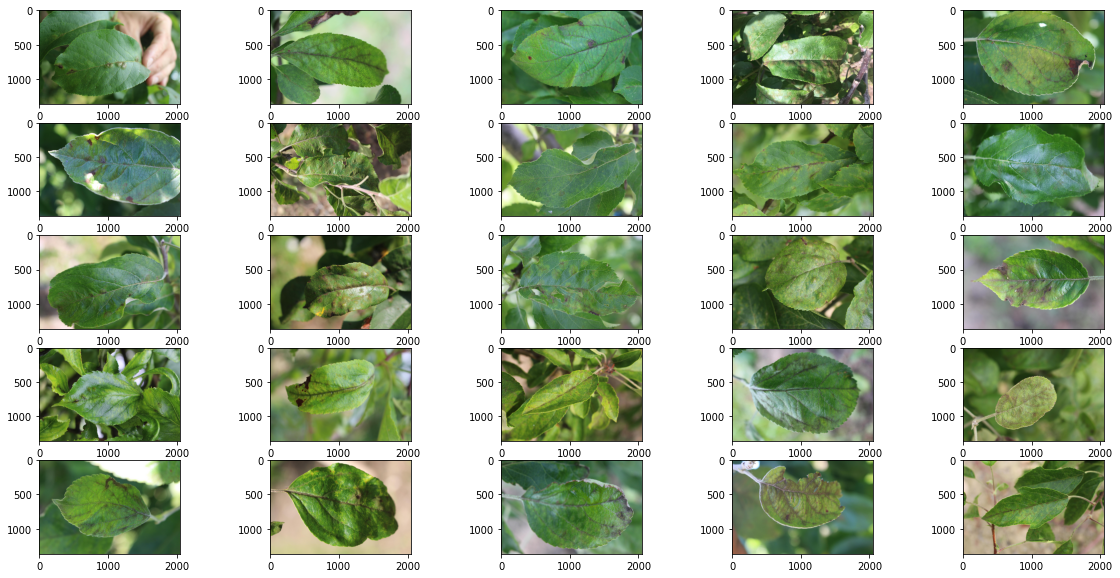
\includegraphics[width=1\linewidth]{images/sample_scab_diseases_leaf.png}
		\caption{Một số mẫu hình ảnh về Scab Diseases Leaf}
		\label{fig:writing-thesis}
	\end{figure}
	\begin{python}
		def plot_patches(data, size_selection, width_size, height_size, figure_size, type_patches=0, is_positive=True):
			if type_patches == 3:
				if is_positive:
					scab_diseases_selection = np.random.choice(
					data[data.scab == 1].index.values, size=size_selection, replace=False)
					for i in range(height_size):
						for j in range(width_size):
							idx = scab_diseases_selection[j + width_size*i]
							image = io.imread(data.loc[idx, 'image_path'])
							ax[i, j].imshow(image)
							ax[i, j].grid(False)
				else:
					non_scab_diseases_selection = np.random.choice(
					data[data.scab == 0].index.values, size=50, replace=False)
					for i in range(height_size):
						for j in range(width_size):
							idx = non_scab_diseases_selection[j + width_size*i]
							image = io.imread(data.loc[idx, 'image_path'])
							ax[i, j].imshow(image)
							ax[i, j].grid(False)
	\end{python}
	\subsection{4.2 Phân phối các kênh màu trên mẫu từ tập dữ liệu}
	\begin{figure}[H]
		\centering
		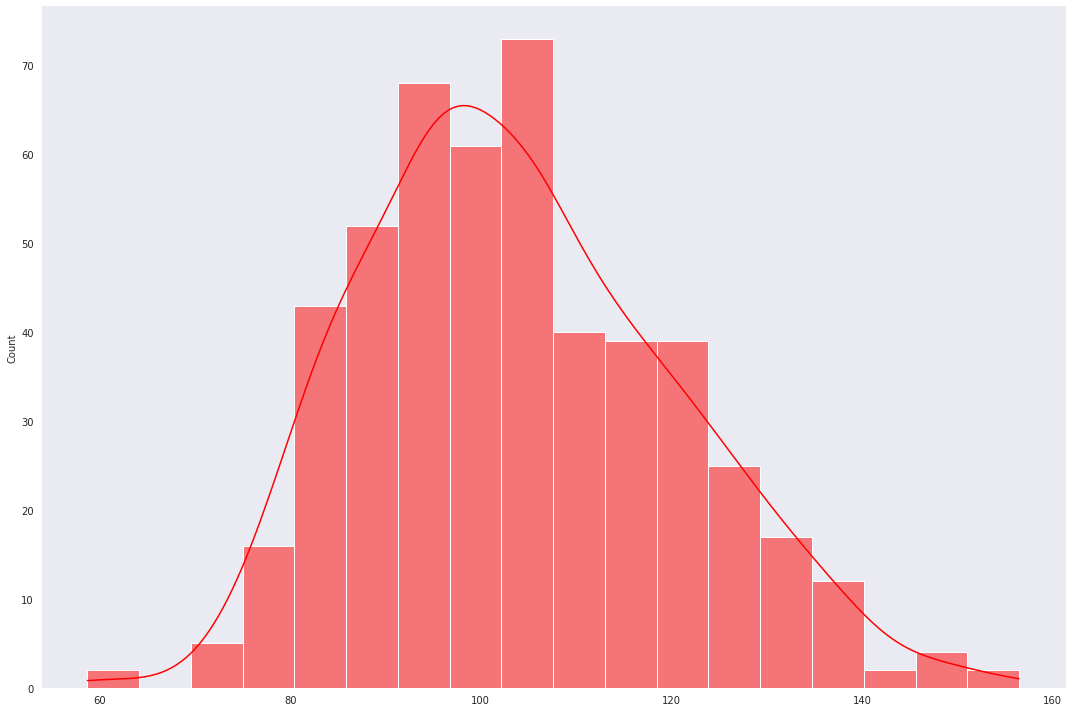
\includegraphics[width=1\linewidth]{images/red_channel_distribution.png}
		\caption{Phân phối kênh màu đỏ - Red Channel Distribution}
		\label{fig:writing-thesis}
	\end{figure}
	\begin{figure}[H]
		\centering
		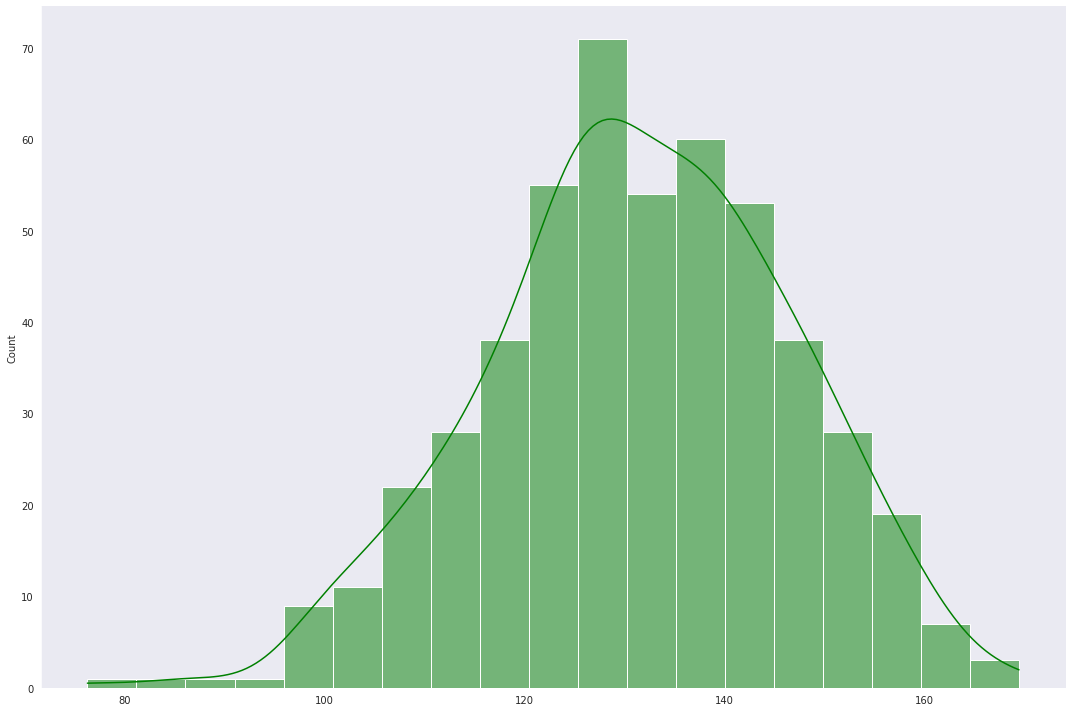
\includegraphics[width=1\linewidth]{images/green_channel_distribution.png}
		\caption{Phân phối kênh màu xanh lá - Green Channel Distribution}
		\label{fig:writing-thesis}
	\end{figure}
	\begin{figure}[H]
		\centering
		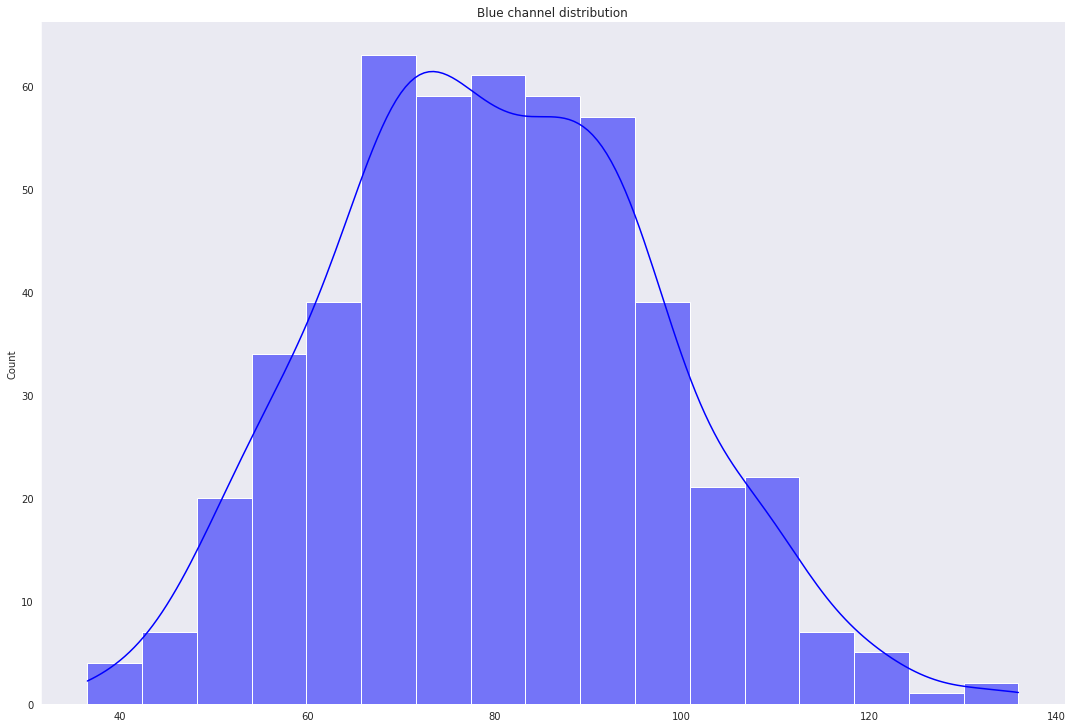
\includegraphics[width=1\linewidth]{images/blue_channel_distribution.png}
		\caption{Phân phối kênh màu xanh dương - Blue Channel Distribution}
		\label{fig:writing-thesis}
	\end{figure}
	\begin{figure}[H]
		\centering
		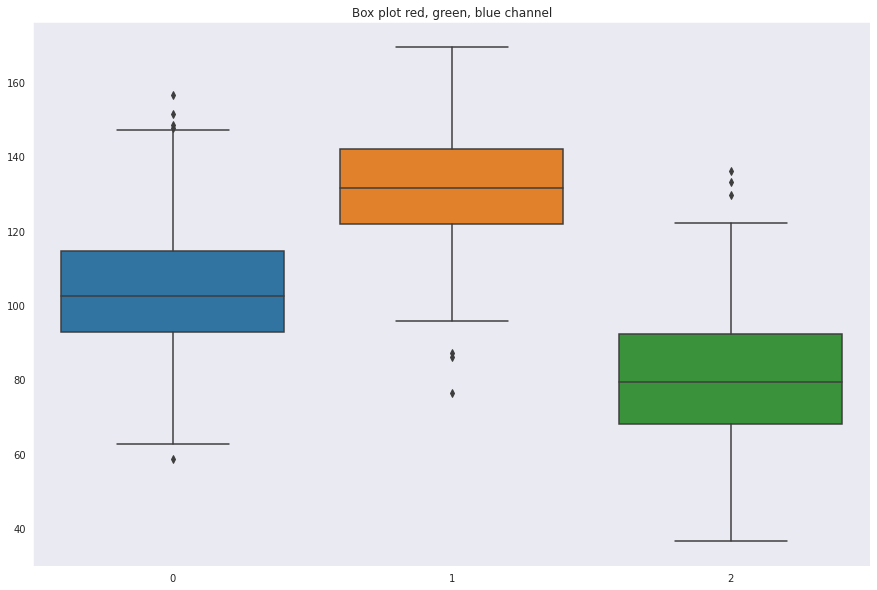
\includegraphics[width=1\linewidth]{images/boxplot_channels_distribution.png}
		\caption{So sánh những kênh màu}
		\label{fig:writing-thesis}
	\end{figure}
	\subsection{4.3 Trực quan hóa mục tiêu}
	\begin{figure}[H]
		\centering
		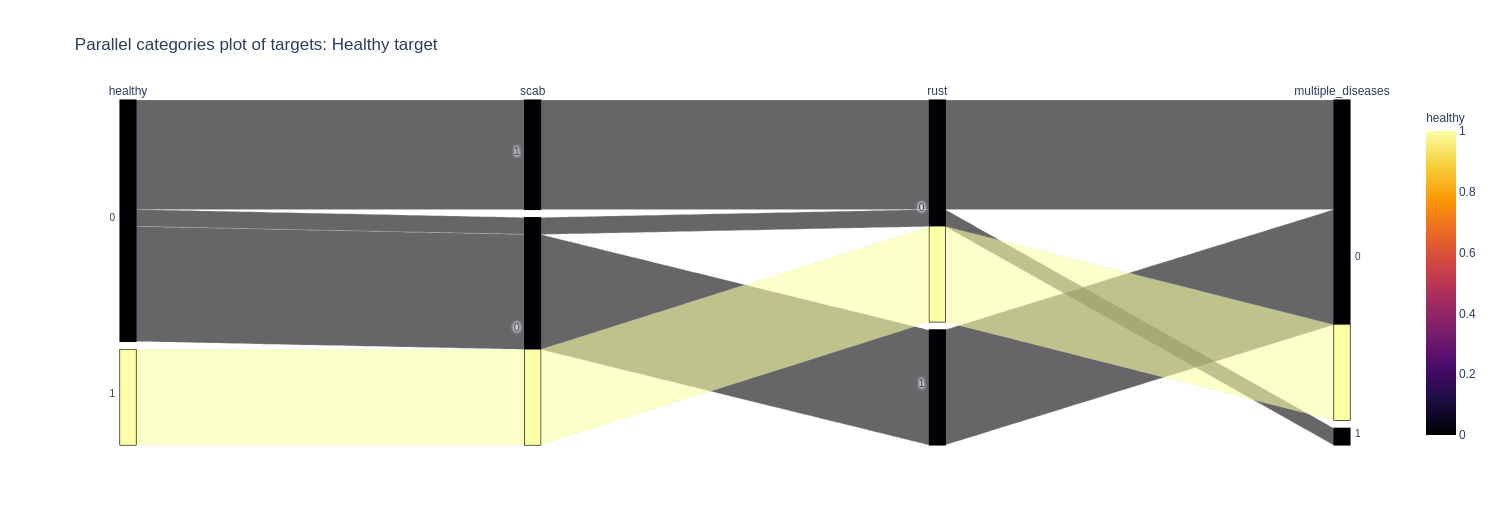
\includegraphics[width=1\linewidth]{images/parallel_categories_healthy_target.png}
		\caption{Biểu đồ loại song song - highlight Healthy Category}
		\label{fig:writing-thesis}
	\end{figure}
	\begin{figure}[H]
		\centering
		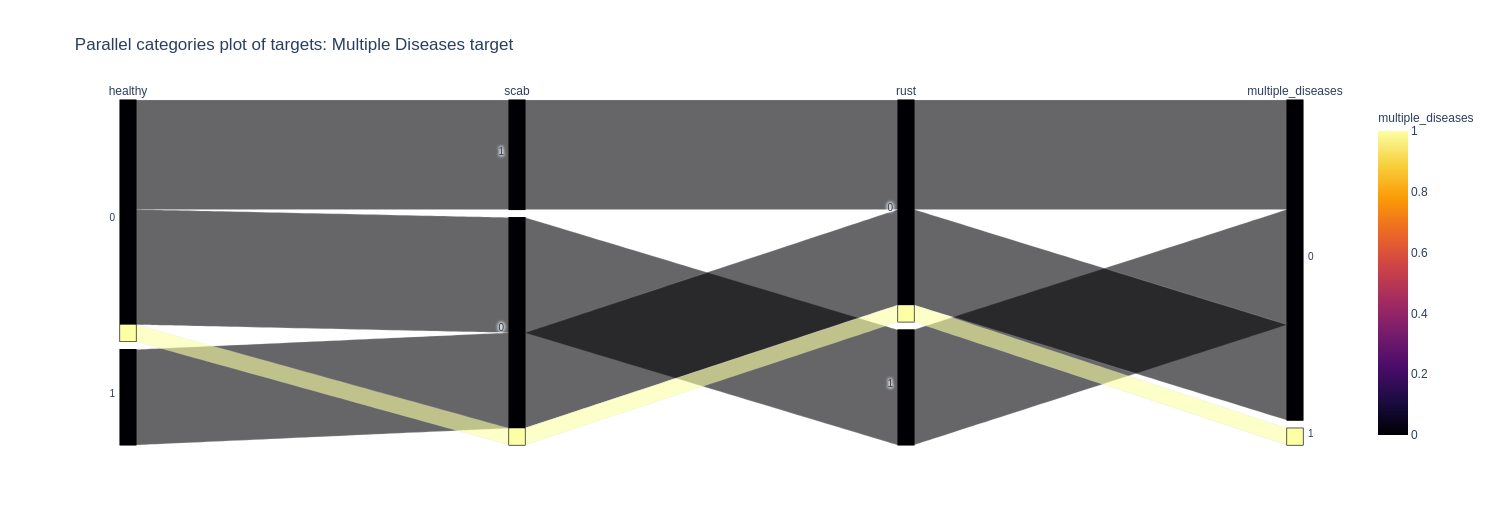
\includegraphics[width=1\linewidth]{images/parallel_categories_multiple_deseases.png}
		\caption{Biểu đồ loại song song - highlight Multiple Diseases Category}
		\label{fig:writing-thesis}
	\end{figure}
	\begin{figure}[H]
		\centering
		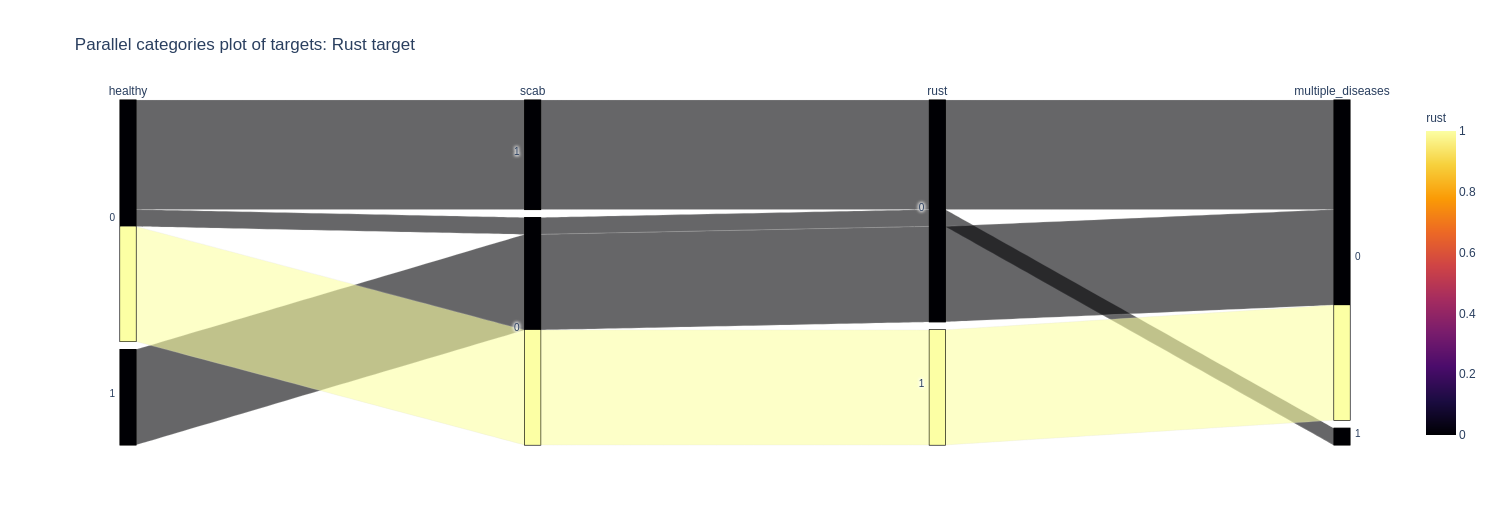
\includegraphics[width=1\linewidth]{images/parallel_categories_rust_target.png}
		\caption{Biểu đồ loại song song - highlight Rust Category}
		\label{fig:writing-thesis}
	\end{figure}
	\begin{figure}[H]
		\centering
		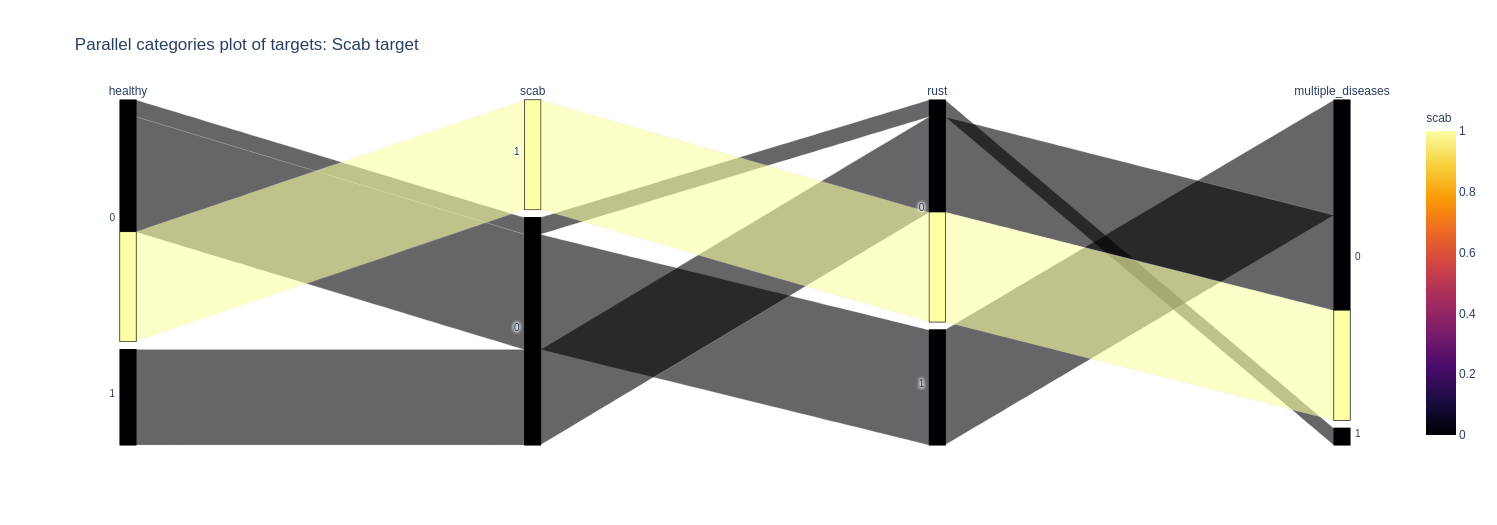
\includegraphics[width=1\linewidth]{images/parallel_categories_scab_target.png}
		\caption{Biểu đồ loại song song - highlight Scab Category}
		\label{fig:writing-thesis}
	\end{figure}
	\begin{figure}[H]
		\centering
		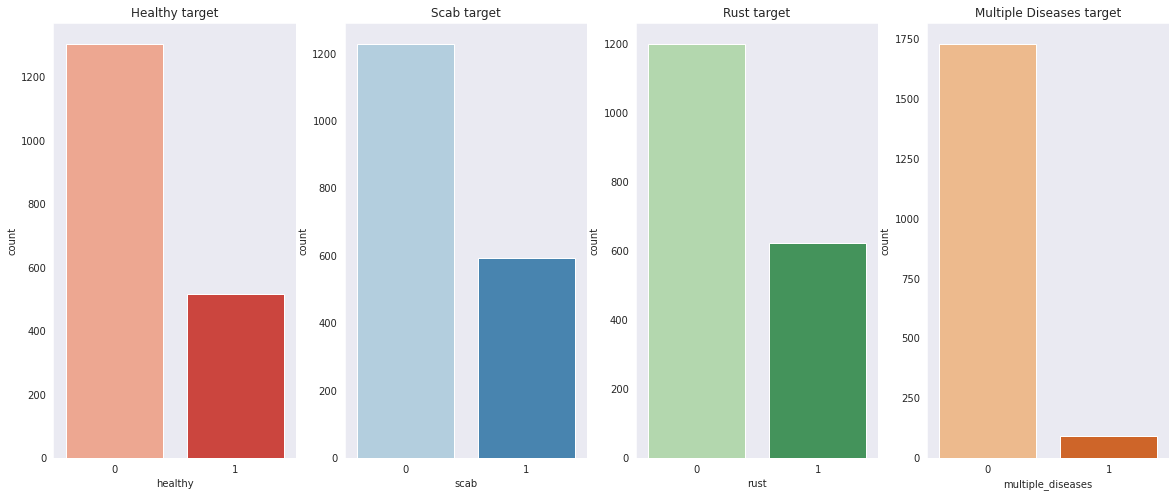
\includegraphics[width=1\linewidth]{images/counting_plot_target.png}
		\caption{Đếm số lượng Healthy - Multiple Diseases - Rust - Scab}
		\label{fig:writing-thesis}
	\end{figure}
	\begin{figure}[H]
		\centering
		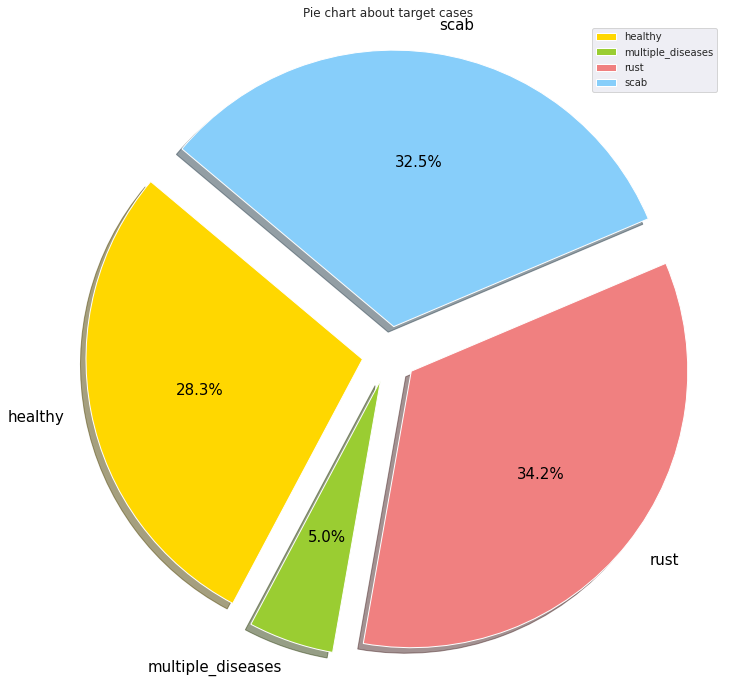
\includegraphics[width=.75\linewidth]{images/pie_chart_targer_plot.png}
		\caption{Biểu đồ phần trăm tỉ lệ các loại bệnh}
		\label{fig:writing-thesis}
	\end{figure}
	\section{5. Xử lý và tăng cường hình ảnh}
	\subsection{5.1 Xác định biên cạnh bằng Canny - The Canny Edge Detection}
	\begin{python}
		def canny_edge_detection(image_path, low_threshold=100, high_threshold=200, figsize=(30, 20)):
			# Read image from image_path
			image = io.imread(image_path)
			
			# copy from image to embed image
			embed_image = image.copy()
			
			# Apply Canny Edges Detection with low_threshold and high_threshold
			canny_edges = cv.Canny(image, low_threshold, high_threshold)
			edge_coors = []
			for i in range(canny_edges.shape[0]):
				for j in range(canny_edges.shape[1]):
					if canny_edges[i][j] != 0:
						edge_coors.append((i, j))
			
			# Bounding box detection
			# (row_min, row_min) -> (col_min, col_maxn)
			embed_image[edge_coors[np.argsort([coor[0] for coor in edge_coors])[0]][0]-10:edge_coors[np.argsort([coor[0] for coor in edge_coors])[0]][0]+10, edge_coors[np.argsort([coor[1] for coor in edge_coors])[0]][1]:edge_coors[np.argsort([coor[1] for coor in edge_coors])[-1]][1]] = [255, 0, 0]
			
			# (row_max, row_max) -> (col_min, col_max)
			embed_image[edge_coors[np.argsort([coor[0] for coor in edge_coors])[-1]][0]-10:edge_coors[np.argsort([coor[0] for coor in edge_coors])[-1]][0]+10, edge_coors[np.argsort([coor[1] for coor in edge_coors])[0]][1]:edge_coors[np.argsort([coor[1] for coor in edge_coors])[-1]][1]] = [255, 0, 0]
			
			# (row_min, row_max) -> (col_min, col_min)
			embed_image[edge_coors[np.argsort([coor[0] for coor in edge_coors])[0]][0]:edge_coors[np.argsort([coor[0] for coor in edge_coors])[-1]][0], edge_coors[np.argsort([coor[1] for coor in edge_coors])[0]][1]-10: edge_coors[np.argsort([coor[1] for coor in edge_coors])[0]][1]+10] = [255, 0, 0]
			
			# (row_min, row_max) -> (col_max, col_max)
			embed_image[edge_coors[np.argsort([coor[0] for coor in edge_coors])[0]][0]:edge_coors[np.argsort([coor[0] for coor in edge_coors])[-1]][0], edge_coors[np.argsort([coor[1] for coor in edge_coors])[-1]][1]-10:edge_coors[np.argsort([coor[1] for coor in edge_coors])[-1]][1]+10] = [255, 0, 0]
		
			# Show result
			fig, ax = plt.subplots(nrows=1, ncols=3, figsize=figsize)
			ax[0].imshow(image, cmap='gray')
			ax[0].set_title('Original Image', fontsize=24)
			ax[1].imshow(canny_edges, cmap='gray')
			ax[1].set_title('Canny Edges', fontsize=24)
			ax[2].imshow(embed_image, cmap='gray')
			ax[2].set_title('Bounding Box', fontsize=24)
			plt.show()
	\end{python}
	\begin{figure}[H]
		\centering
		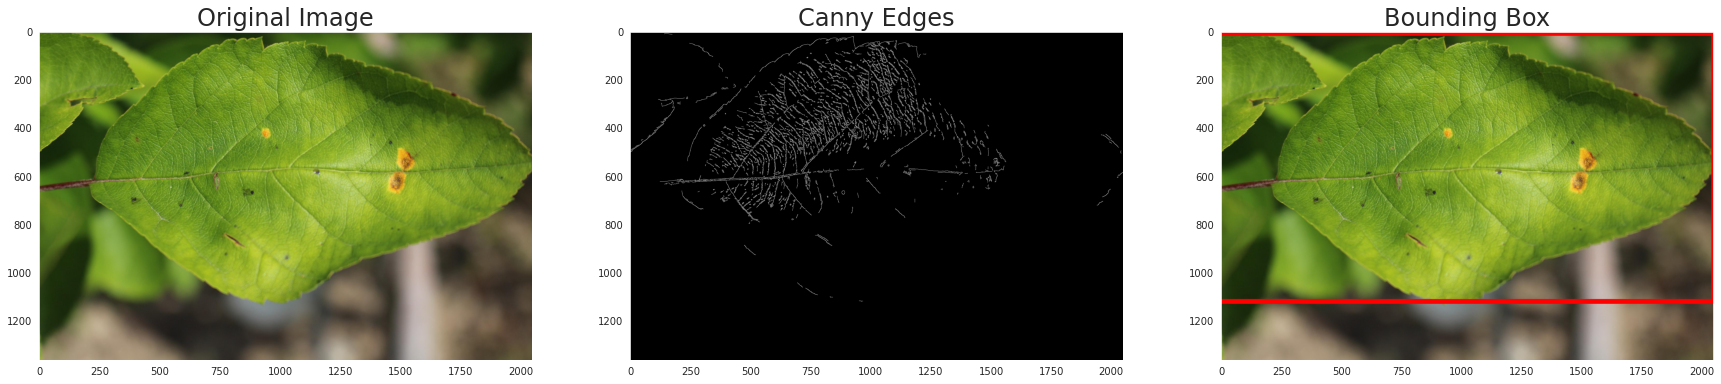
\includegraphics[width=1\linewidth]{images/canny_edge_detector.png}
		\caption{Kết quả giải thuật Canny trên một ảnh ngẫu nhiên}
		\label{fig:writing-thesis}
	\end{figure}
	\begin{figure}[H]
		\centering
		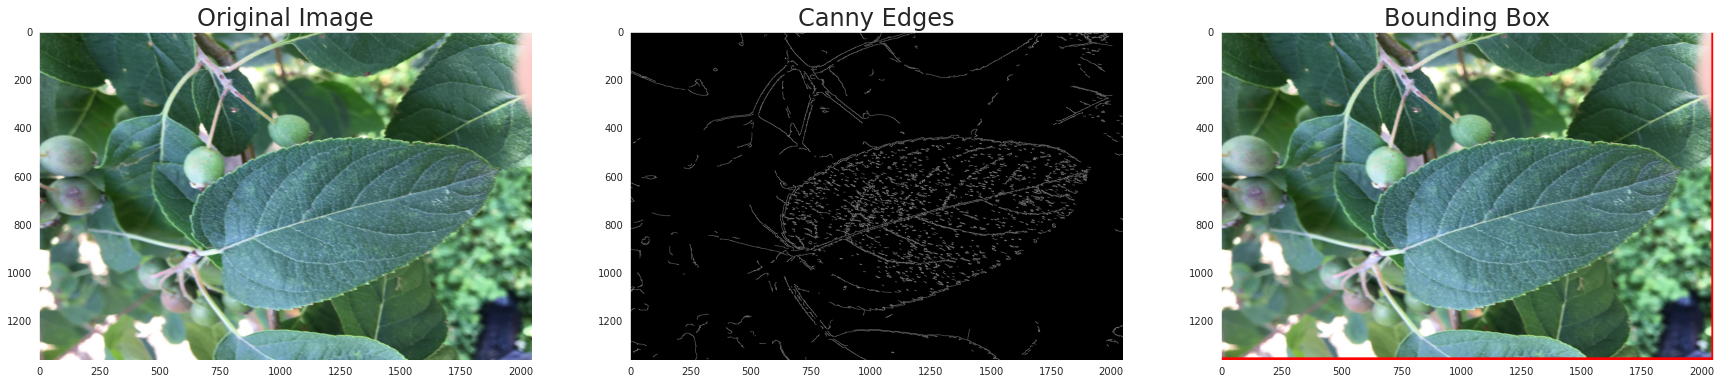
\includegraphics[width=1\linewidth]{images/canny_edge_detector_1.png}
		\caption{Kết quả giải thuật Canny trên một ảnh ngẫu nhiên}
		\label{fig:writing-thesis}
	\end{figure}
	\begin{figure}[H]
		\centering
		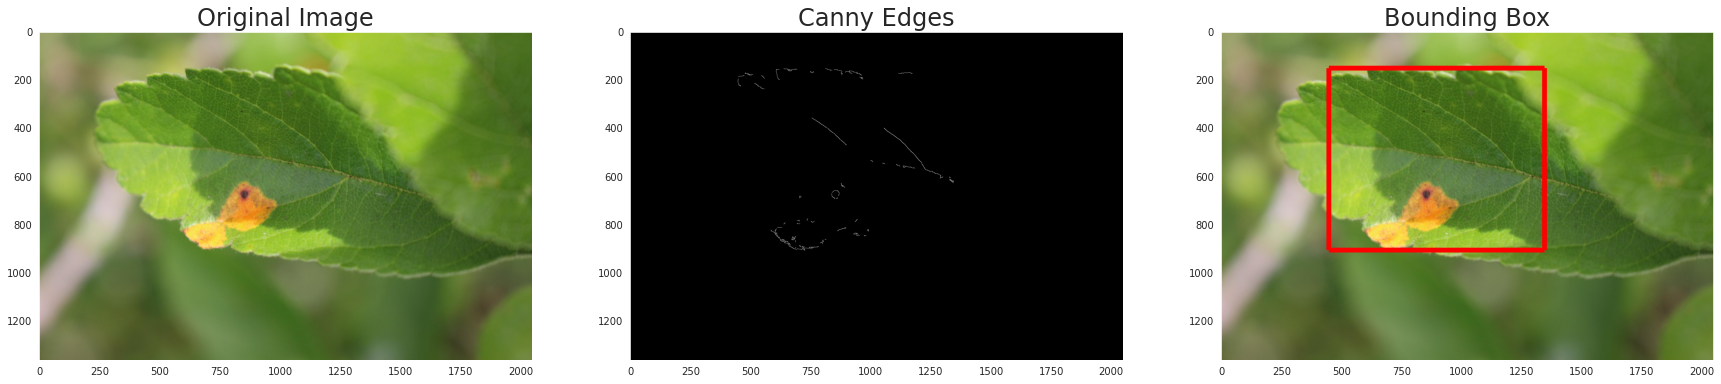
\includegraphics[width=1\linewidth]{images/canny_edge_detector_2.png}
		\caption{Kết quả giải thuật Canny trên một ảnh ngẫu nhiên}
		\label{fig:writing-thesis}
	\end{figure}
	\subsection{5.2 Phép biến đổi lật ảnh - Flipping image}
	\begin{python}
		def flipping_image(image_path, figsize=(30, 20)):
			# Read image from image_path
			image = io.imread(image_path)
			
			# Plotting result when applying cv.flip()
			fig, ax = plt.subplots(nrows=1, ncols=3, figsize=figsize)
			ax[0].imshow(image)
			ax[0].set_title('Original Image', fontsize=24)
			ax[1].imshow(cv.flip(image, 0))
			ax[1].set_title('Vertical Flip', fontsize=24)
			ax[2].imshow(cv.flip(image, 1))
			ax[2].set_title('Horizontal Flip', fontsize=24)
			plt.show()
	\end{python}
	\begin{figure}[H]
		\centering
		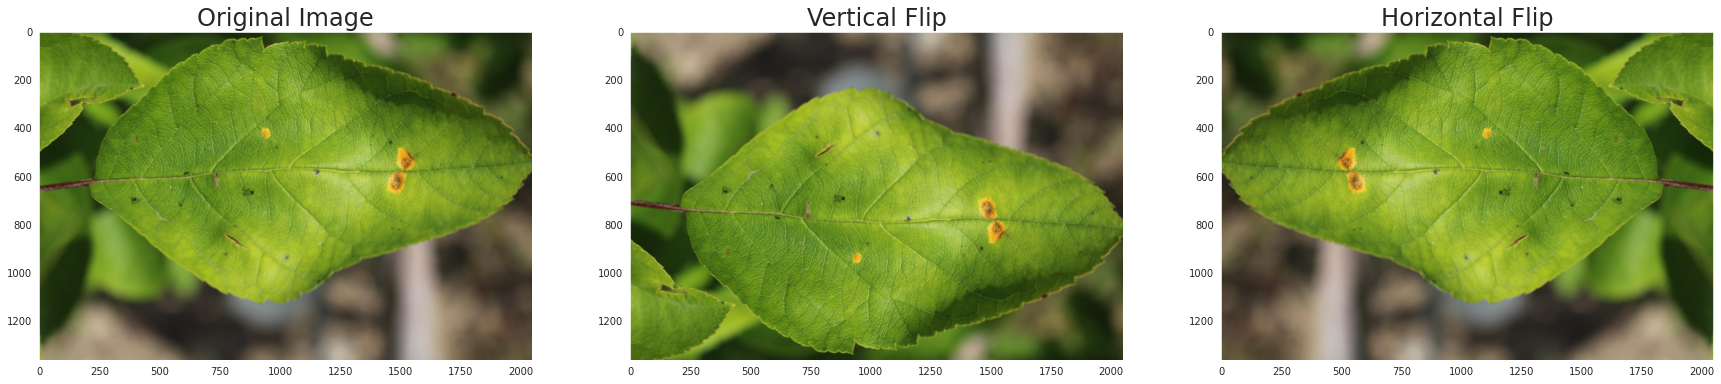
\includegraphics[width=1\linewidth]{images/flipping_image.png}
		\caption{Kết quả phép lật ảnh trên một ảnh ngẫu nhiên}
		\label{fig:writing-thesis}
	\end{figure}
	\begin{figure}[H]
		\centering
		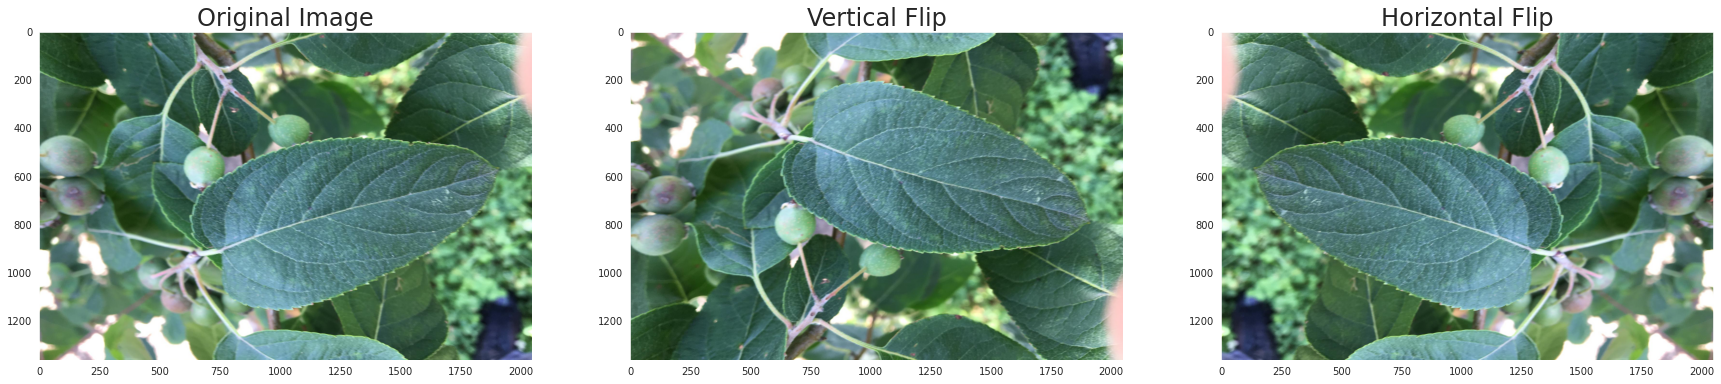
\includegraphics[width=1\linewidth]{images/flipping_image_1.png}
		\caption{Kết quả phép lật ảnh trên một ảnh ngẫu nhiên}
		\label{fig:writing-thesis}
	\end{figure}
	\begin{figure}[H]
		\centering
		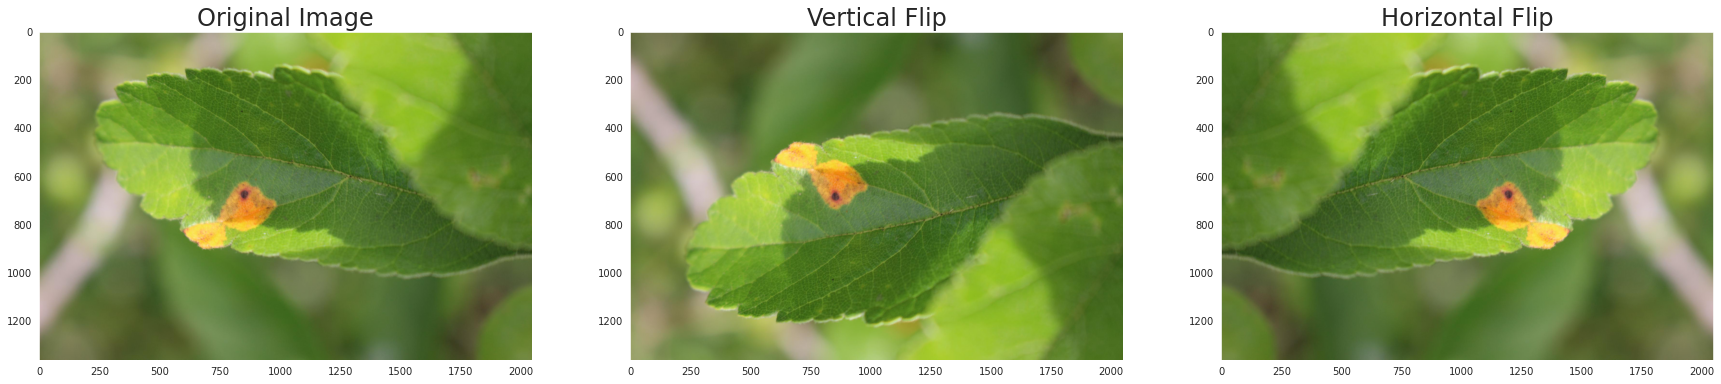
\includegraphics[width=1\linewidth]{images/flipping_image_2.png}
		\caption{Kết quả phép lật ảnh trên một ảnh ngẫu nhiên}
		\label{fig:writing-thesis}
	\end{figure}
	\subsection{5.3 Phép tích chập trên ảnh - Convolutional}
	\begin{python}
		def convolution(image_path, kernel=np.ones((7, 7), np.float32)/25, figsize=(20, 20)):
			# Read image from image_path
			image = io.imread(image_path)
			
			# Initialization figure image
			fig, ax = plt.subplots(nrows=1, ncols=2, figsize=figsize)
			
			# Apply cv filter 2D with kernel with default 7 x 7 Gaussian
			conv = cv.filter2D(image, -1, kernel)
			
			# Plotting result
			ax[0].imshow(image)
			ax[0].set_title('Original Image', fontsize=24)
			ax[1].imshow(conv)
			ax[1].set_title('Convolved Image', fontsize=24)
			plt.show()
	\end{python}
	\begin{figure}[H]
		\centering
		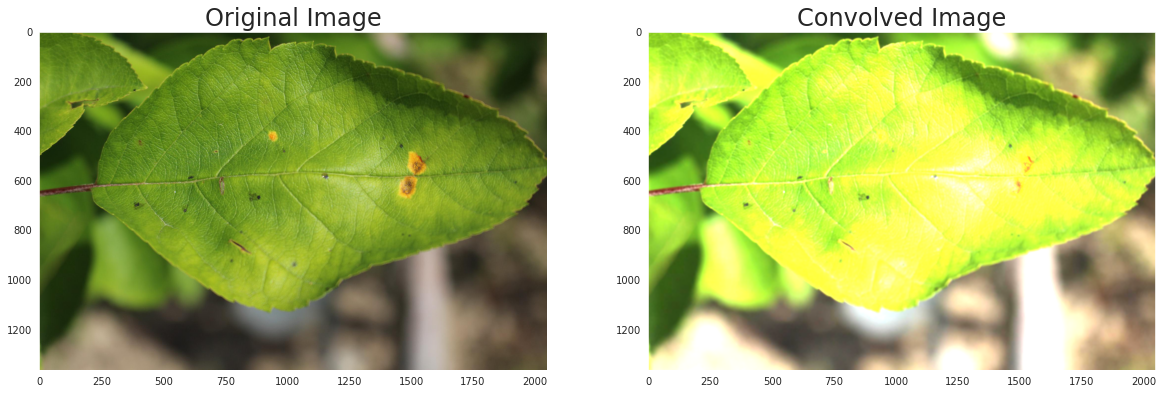
\includegraphics[width=1\linewidth]{images/conv.png}
		\caption{Kết quả phép tích chập trên một ảnh ngẫu nhiên}
		\label{fig:writing-thesis}
	\end{figure}
	\begin{figure}[H]
		\centering
		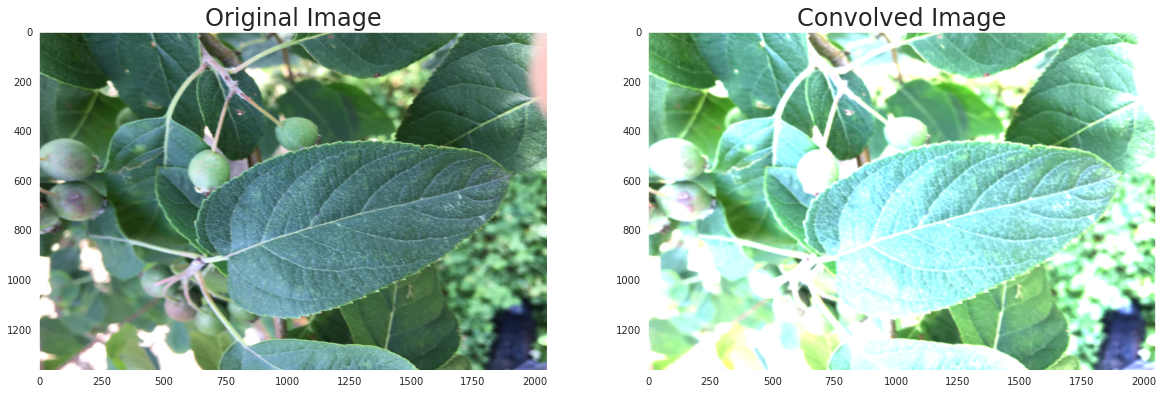
\includegraphics[width=1\linewidth]{images/conv_1.png}
		\caption{Kết quả phép tích chập trên một ảnh ngẫu nhiên}
		\label{fig:writing-thesis}
	\end{figure}
	\begin{figure}[H]
		\centering
		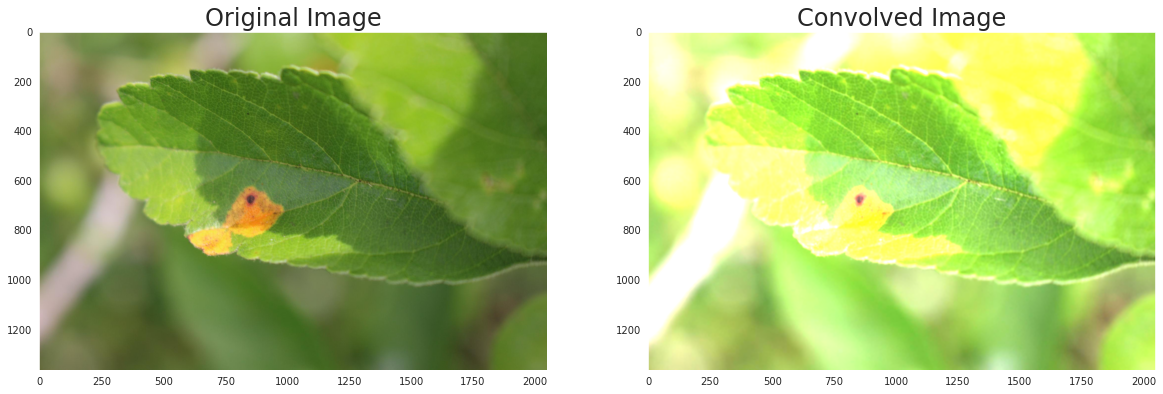
\includegraphics[width=1\linewidth]{images/conv_2.png}
		\caption{Kết quả phép tích chập trên một ảnh ngẫu nhiên}
		\label{fig:writing-thesis}
	\end{figure}
	\subsection{5.4 Làm trơn ảnh - Bluring image}
	\begin{python}
		def blur_image(image_path, kernel_width=100, kernel_height=100, figsize=(20, 20)):
			# Read image from image_path
			image = io.imread(image_path)
			
			# Initialization figure image
			fig, ax = plt.subplots(nrows=1, ncols=2, figsize=figsize)
			
			# Plotting result when applying cv.blur()
			ax[0].imshow(image)
			ax[0].set_title('Original Image', fontsize=24)
			ax[1].imshow(cv.blur(image, (kernel_width, kernel_height)))
			ax[1].set_title('Blurred Image', fontsize=24)
			plt.show()
	\end{python}
	\begin{figure}[H]
		\centering
		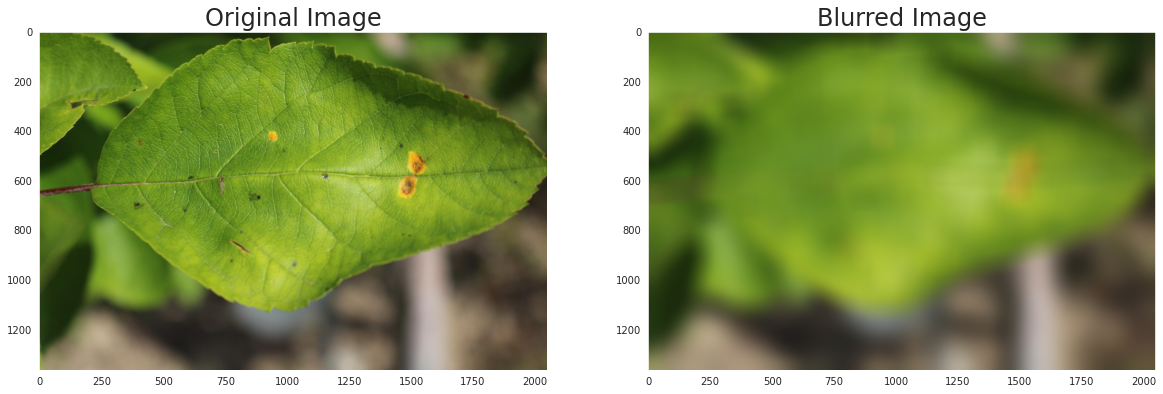
\includegraphics[width=1\linewidth]{images/blur_1.png}
		\caption{Kết quả phép làm trơn ảnh trên một ảnh ngẫu nhiên}
		\label{fig:writing-thesis}
	\end{figure}
	\begin{figure}[H]
		\centering
		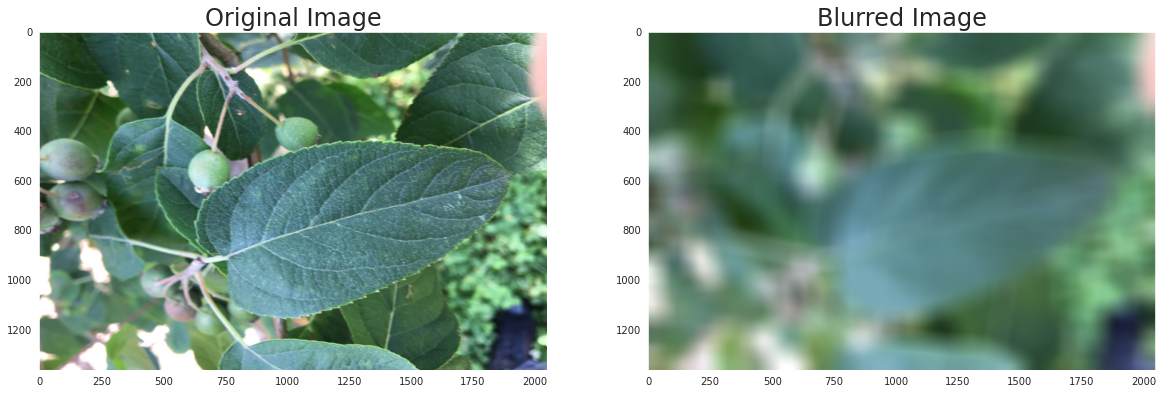
\includegraphics[width=1\linewidth]{images/blur_2.png}
		\caption{Kết quả phép làm trơn ảnh trên một ảnh ngẫu nhiên}
		\label{fig:writing-thesis}
	\end{figure}
	\begin{figure}[H]
		\centering
		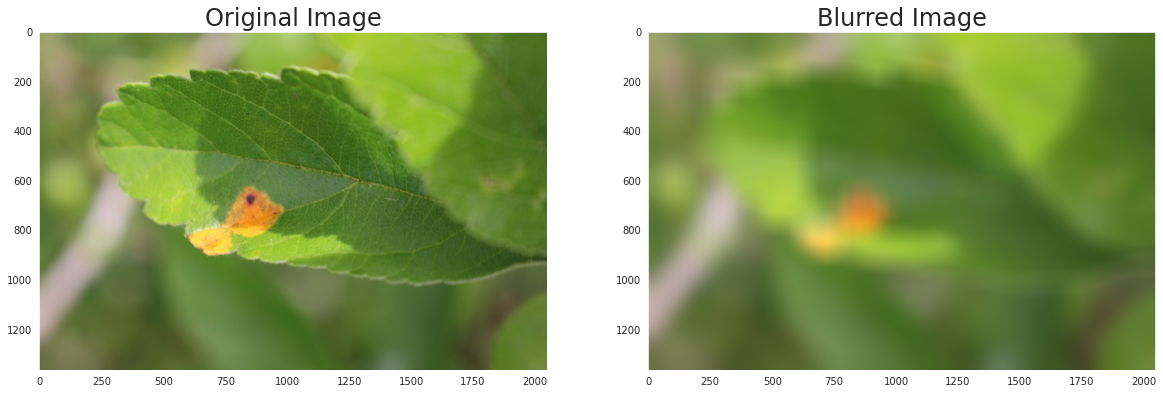
\includegraphics[width=1\linewidth]{images/blur_3.png}
		\caption{Kết quả phép làm trơn ảnh trên một ảnh ngẫu nhiên}
		\label{fig:writing-thesis}
	\end{figure}
	\section{6. Cài đặt Neural Networks}
	
	\section{7. Huấn luyện và đánh giá mô hình Neural Networks}
	
	\section{9. Các kết quả đạt được}
	
	\section{10. Kết luận}
\end{document}